\chapter{Transformer、注意力与科学基础模型概念}

\section{本章导读：注意力机制不是解释性的万能钥匙}

Transformer 和基础模型是现代 AI 的核心入口，但本科教材里最重要的不是追逐最新架构，而是理解它们为什么能处理序列、token、patch 和多模态表示。注意力机制允许模型在输入不同位置之间建立依赖关系，这一点对文本、光谱、时间序列和图像 patch 都有直观意义。

同时，注意力权重并不自动等于科学解释，基础模型输出也不自动等于可信结论。大模型可能表现很强，却更需要数据边界、训练来源、迁移适用性和验证流程。越是强大的模型，越不能绕过 baseline 和错误复查。

读这一章时，请把 Transformer 当成一种表示学习框架来理解，而不是把它当成万能方法。真正要带走的是：什么任务需要长程依赖或上下文建模，什么证据能说明模型迁移到了你的科学问题上。

\section{案例目标}

到这里为止，Part V 已经建立了三块地基：神经网络的非线性表达能力、卷积对局部模式的适配性，以及自编码器对低维表示的压缩能力。接下来，我们需要再补上一条现代 AI 的核心主线：\textbf{模型能不能在更长的序列里，按内容和位置动态决定“现在该看哪里”？}

本章的目标有三点：

\begin{enumerate}
    \item 理解为什么 bag-of-features 或简单平均在序列任务里经常不够；
    \item 理解注意力（attention）如何扮演“动态读出相关 token”的角色；
    \item 理解 Transformer 和科学基础模型为什么能统一处理文本、图像 patch、光谱片段和时间序列块。
\end{enumerate}

\section{为什么卷积之后还需要注意力}

卷积非常适合提取局部模式，但它默认最擅长回答的是“这个局部窗口里有什么”。一旦任务变成：

\begin{itemize}
    \item 某个 patch 应该和更远处哪个 patch 对齐；
    \item 某条谱线的解释要结合更长范围的上下文；
    \item 某个时间序列片段是否重要，要看它和别处是否形成配对结构；
\end{itemize}

模型就需要一种更灵活的机制：不是固定看邻近位置，而是\textbf{根据当前问题，动态决定该从整段序列中读取哪些 token。}

这正是注意力机制的重要性所在。它不是简单的平均，也不是固定卷积核，而是一种“按当前查询选择上下文”的读出方式。

\section{一个极小的 token 化光谱教学数据集}

配套 notebook 使用 \nolinkurl{spectral_token_attention_demo.csv}。它不是原始 flux 数据，而是一个\textbf{教学版 token 序列数据集}。每个样本包含 6 个按顺序排列的 token：

\begin{itemize}
    \item \texttt{sample\_id}；
    \item \texttt{split}；
    \item \texttt{sequence\_label}；
    \item \texttt{tok00} 到 \texttt{tok05} 的 token 序列。
\end{itemize}

这些 token 可以被理解为非常粗糙的光谱 patch 标签，例如：

\begin{itemize}
    \item \texttt{blue\_continuum}；
    \item \texttt{red\_continuum}；
    \item \texttt{ha\_emission}；
    \item \texttt{balmer\_absorption}；
    \item \texttt{sky\_residual}；
    \item \texttt{center\_mark}。
\end{itemize}

这个数据集的关键设计非常刻意：\textbf{所有类别都包含同样的一组 token，多重集合完全相同；唯一的差别，是哪一个 token 紧跟在 \texttt{center\_mark} 之后。}

因此：

\begin{itemize}
    \item 如果模型只统计“有哪些 token”，三个类别看起来完全一样；
    \item 如果模型能读出“\texttt{center\_mark} 后面的那个 token 是谁”，它就能立刻分辨发射上下文、吸收上下文和伪迹上下文。
\end{itemize}

配套 notebook 的后半段还会额外引入第二个教学数据集：\nolinkurl{spectral_masked_token_workflow_demo.csv}。

这组小数据把序列长度扩到 8 个 token，并在固定位置放入 \texttt{[MASK]}。clean 样本要求模型从更远处的 anchor token 读回被遮住的目标 token；review 样本则故意加入 blend token 或第二个 mask，让学生看到 masked-token workflow 也需要人工复核队列。

\section{先看 bag-of-tokens baseline}

为了保持全书一致的 baseline 思维，notebook 先做一个最朴素的 bag-of-tokens 表示：对每个 token 计数，然后做最近中心分类。最小形式可以写成：

\begin{examplebox}[bag-of-tokens baseline]
\begin{lstlisting}[style=pythonstyle]
feature[token] = count_in_sequence(token)
\end{lstlisting}
\end{examplebox}

在这个教学数据上，bag-of-tokens baseline 的测试集准确率只有 \texttt{0.33}。这并不奇怪，因为三个类别的 token 计数向量完全相同，模型失去了所有顺序信息。表~\ref{tab:ch34_bag_vs_attention} 把它与 patch token 和位置感知注意力头放在同一个最小对照中。

\begin{table}[htbp]
\centering
\small
\resizebox{\textwidth}{!}{
\begin{tabular}{p{0.23\textwidth}ccp{0.33\textwidth}}
\toprule
方法 & 测试集准确率 & 读出的关键信息 & 教学解读 \\
\midrule
bag-of-tokens 最近中心 & 0.33 & 只有 token 计数 & 顺序被抹掉，同一组 token 无法区分类别 \\
bag-of-2-patches 最近中心 & 1.00 & 两个相邻 token 组成的局部 patch motif & patch token 把一小段局部顺序压进 token 身份里 \\
位置感知注意力头 & 1.00 & \texttt{center\_mark} 后面的相关 token & 用动态读出保留“现在该看哪里”这件事 \\
\bottomrule
\end{tabular}
}
\caption{本章教学 notebook 中的三个最小对照组。这里的重点不是追求高分，而是直接暴露顺序信息、局部 patch 化和动态读出在序列建模中的不同作用。}
\label{tab:ch34_bag_vs_attention}
\end{table}

\subsection*{从 token 到 patch token}

更新后的 notebook 还把同一条 6-token 序列按宽度 2 重新切成 3 个 patch token。例如，原来局部片段里的 \texttt{center\_mark} 与后一位 token 会被压成一个新的 patch token。对发射类样本来说，这个局部 motif 可以写成 \texttt{center\_mark|ha\_emission}；吸收类和伪迹类则会得到对应的变体。

在这个教学数据上，bag-of-2-patches 最近中心也能达到 \texttt{1.00}。这并不是因为它“比 attention 更强”，而是因为类别线索刚好被压进了同一个局部 patch motif。它提供了一个很重要的过渡直觉：在视觉、光谱和时间序列 Transformer 里，patch token 往往先保留一小段局部顺序，再让 attention 去读取 patch 与 patch 之间的全局关系。

\section{注意力到底在做什么}

标准缩放点积注意力（scaled dot-product attention）的最小形式可以写成：

\begin{examplebox}[一个最小注意力公式]
\begin{lstlisting}[style=pythonstyle]
score_i = (q · k_i) / sqrt(d)
weight_i = softmax(score_i)
context = sum(weight_i * v_i for i in tokens)
\end{lstlisting}
\end{examplebox}

这里的三类对象分别扮演不同角色：

\begin{itemize}
    \item query（查询）回答“当前想找什么”；
    \item key（键）回答“每个 token 是否值得被关注”；
    \item value（值）回答“如果关注这个 token，应当读出什么信息”。
\end{itemize}

也就是说，注意力不是在对整段序列做统一平均，而是在问：\textbf{对于当前这个查询，哪几个 token 应该获得更高权重？}

\section{为什么位置编码很重要}

如果只有 token 身份、没有位置编码，那么本章数据里的三类样本仍然是不可分的：因为它们包含同样的 token 集合。模型需要知道的不只是“出现了 \texttt{ha\_emission}”，而是“\texttt{ha\_emission} 出现在了 \texttt{center\_mark} 后面还是后更远的位置”。

这就是 Transformer 里位置编码的重要性。它把“这个 token 是谁”和“这个 token 在哪里”合并起来，使模型能够同时感知内容与顺序。

图~\ref{fig:ch34_attention_sequence} 展示了本章教学数据里的核心几何直觉：真正应该被读出的，不是整段序列的平均，而是围绕 \texttt{center\_mark} 的相关上下文。

\begin{figure}[htbp]
\centering
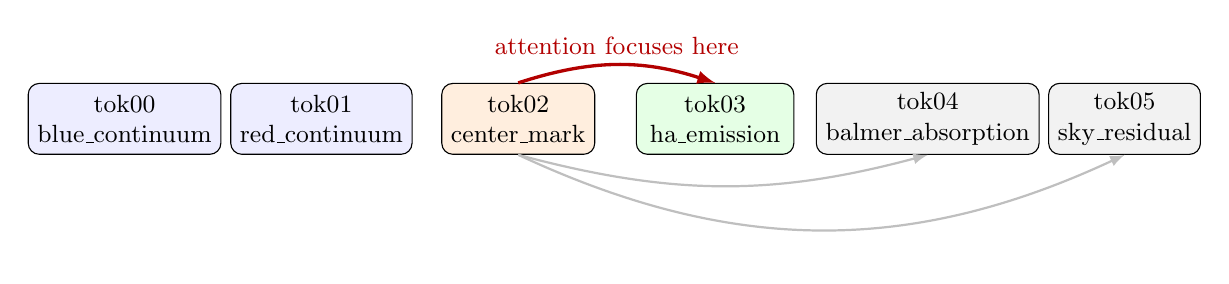
\begin{tikzpicture}[every node/.style={font=\small, align=center}, >=latex]
\node[draw, rounded corners, fill=blue!7, minimum width=2.1cm, minimum height=0.9cm] (t0) at (0,0) {tok00\\blue\_continuum};
\node[draw, rounded corners, fill=blue!7, minimum width=2.0cm, minimum height=0.9cm] (t1) at (2.5,0) {tok01\\red\_continuum};
\node[draw, rounded corners, fill=orange!13, minimum width=1.8cm, minimum height=0.9cm] (t2) at (5.0,0) {tok02\\center\_mark};
\node[draw, rounded corners, fill=green!10, minimum width=2.0cm, minimum height=0.9cm] (t3) at (7.5,0) {tok03\\ha\_emission};
\node[draw, rounded corners, fill=gray!10, minimum width=2.2cm, minimum height=0.9cm] (t4) at (10.2,0) {tok04\\balmer\_absorption};
\node[draw, rounded corners, fill=gray!10, minimum width=1.9cm, minimum height=0.9cm] (t5) at (12.7,0) {tok05\\sky\_residual};

\draw[->, very thick, red!70!black, bend left=18] (t2.north) to node[above] {attention focuses here} (t3.north);
\draw[->, thick, gray!50, bend right=15] (t2.south) to (t4.south);
\draw[->, thick, gray!50, bend right=25] (t2.south) to (t5.south);
\end{tikzpicture}
\caption{本章教学序列中的一个代表性样本。真正决定标签的是 \texttt{center\_mark} 后面最相关的 token，而不是整段 token 集合的无差别平均。}
\label{fig:ch34_attention_sequence}
\end{figure}

\section{再往前一步：一个最小 masked-token workflow}

notebook 的第二段不再做上下文分类，而是改成一个最小 masked-token 任务。配套数据是一个新的 masked-token workflow demo 表，包含：

\begin{itemize}
    \item \texttt{sample\_id}；
    \item \texttt{split\_role}；
    \item \texttt{quality\_flag}；
    \item \texttt{target\_token}；
    \item \texttt{tok00} 到 \texttt{tok07} 的 token 序列。
\end{itemize}

这里的关键设计同样是刻意的：所有 clean 样本在观测到的 token 多重集合上仍然完全相同，只有更远处那个 anchor token 的身份不同。也就是说，如果模型对位置不敏感，它仍然只能退化成一个 \texttt{0.33} 的 mask-blind baseline；只有当查询能够跨位置跳到正确的 anchor 上时，才可能稳定恢复被遮住的目标 token。

在更新后的 notebook 里，这个 masked-token workflow 分成三步。第一步仍然保留一个 hand-crafted 的位置感知 masked-token 头，直接把查询跳到 \texttt{tok06} 的 anchor token 上，用它建立“注意力究竟在读哪里”的直觉；这个版本在 clean test 上达到 \texttt{1.00}，并通过 validation 置信度阈值把 2 个 review 样本送入 \texttt{manual\_review}。

第二步先训练一个\textbf{纯 Python、单头、低维的 tiny self-attention masked-token learner}。它只保留 token embedding、position embedding、一个可训练 attention 头和 3 类输出投影，不依赖 NumPy、PyTorch 或大模型库。在固定随机种子下训练 50 个 epoch 后，这个 tiny learner 同样在 clean validation/test 上达到 \texttt{1.00}，并把 validation-calibrated ready threshold 校准到 \texttt{0.979}，继续把 \texttt{R\_blend} 与 \texttt{R\_mask} 两个 held-out review 样本送回 \texttt{manual\_review}。

第三步再把同一任务扩展到一个\textbf{纯 Python、双头的 masked-token learner}。这个 two-head 版本保留共享 token/position embedding，但用两个可训练 attention 头共同读出 3 类 logits。在固定随机种子下训练 60 个 epoch 后，它在 clean validation/test 上同样达到 \texttt{1.00}，validation loss 约为 \texttt{0.0308}，clean-test loss 约为 \texttt{0.0080}，并把 validation-calibrated ready threshold 校准到 \texttt{0.901}。6 个 clean test 样本全部留在 auto-ready 路径，而 \texttt{R\_blend} 与 \texttt{R\_mask} 继续被送回 \texttt{manual\_review}。注意力快照还显示，一个 head 常去读 \texttt{tok05} / \texttt{tok01} 之类的支持位置，另一个 head 更常锁定 \texttt{tok06} 的长程 anchor。

notebook 最后再多接一个\textbf{masked-patch pretraining objective}。这一次配套数据不再是 8 个单 token，而是一个新的 \texttt{spectral\_masked\_patch\_workflow\_demo.csv}：每条序列包含 5 个 patch tokens，其中 \texttt{patch02} 固定为 \texttt{[MASK\_PATCH]}，真正决定目标 patch 的锚点则被放在 \texttt{patch04}。更重要的是，clean rows 在\emph{可见 patch 的多重集合上仍然完全相同}，所以 bag-of-visible-patches baseline 会再次退化到 \texttt{0.33}；只有把查询从 mask patch 动态读到 \texttt{patch04}，才能稳定恢复 3 类 \texttt{center\_mark|*} 中心 patch。

在这组新数据上，notebook 继续训练一个纯 Python 的 two-head masked-patch learner。它在固定随机种子下训练 60 个 epoch 后，在 clean validation/test 上同样达到 \texttt{1.00}，validation-calibrated ready threshold 约为 \texttt{0.977}；6 个 clean test patches 全部保留在 auto-ready 路径，2 个 held-out review rows 则继续回到 \texttt{manual\_review}。从教学上看，这一步的重要意义不是“再多做一道分类题”，而是让学生第一次把\textbf{patch token、multi-head attention 和 masked-patch pretraining objective} 放进同一条最小可训练链里。

\section{配套 notebook 做了什么}

本章 notebook 采用的是一个非常克制的 teaching-first 版本：

\begin{itemize}
    \item 先读取 token 序列数据，并打印各类别代表样本；
    \item 用 bag-of-tokens 最近中心做 baseline；
    \item 再实现一个最小位置感知注意力头；
    \item 把同一条 6-token 序列再改写成宽度为 2 的 patch tokens，对比 bag-of-patches 会保留什么局部顺序；
    \item 比较两种方法在测试集上的准确率和混淆情况；
    \item 打印注意力权重，直接展示模型把权重放到了哪里；
    \item 再读取第二组 masked-token workflow 数据，先写一个 hand-crafted masked-token 头，再训练一个纯 Python 的单头 tiny self-attention learner，并继续扩到一个 two-head extension；
    \item 最后再读取第三组 masked-patch workflow 数据，用同样的 two-head tiny attention 骨架去恢复整个中心 patch；
    \item 用 validation 置信度校准 ready threshold，检查这些 trainable learner 是否自己把注意力学到 \texttt{tok06}，并把 held-out 样本路由到 masked-prediction-ready 或 manual-review。
\end{itemize}

notebook 里仍然没有训练大模型，也没有堆叠多层 block。它只是把一个单头、低维、几十个样本级更新就能收敛的 teaching-size masked-token learner，再推进到一个同样极小的 two-head extension，并最后补上一条 masked-patch objective。重点还是同一个：让学生先理解\textbf{注意力是一种动态读出机制，而 patch token、multi-head attention 与 masked-token / masked-patch objective 只是把这种读出接回更接近真实 Transformer 的表示与预训练入口。}

\section{怎样从这里走向 Transformer}

更新后的 notebook 已经把三步过渡接回来了：先把 token 序列 patchify，再把单头 learner 扩成一个最小 two-head 版本，最后把整条链接到一个真正的 masked-patch objective 上。不过，真实的 Transformer 还会继续扩展成更完整的结构：

\begin{itemize}
    \item 多头注意力（multi-head attention）同时从不同角度读取上下文；
    \item 前馈层（feed-forward layers）在每个位置上进一步变换表示；
    \item 残差连接和层归一化帮助更深的网络稳定训练；
    \item 大规模预训练让模型先学到普遍的 token 关系，再迁移到具体任务。
\end{itemize}

图~\ref{fig:ch34_foundation_pipeline} 给出了从教学 attention 到科学基础模型的最小概念链。

\begin{figure}[htbp]
\centering
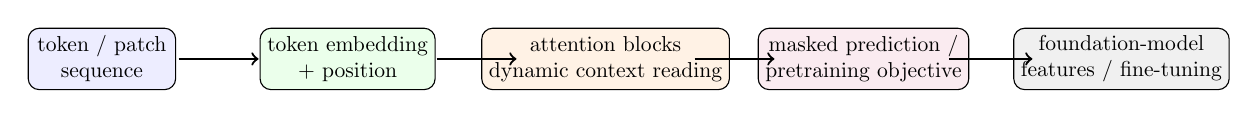
\begin{tikzpicture}[every node/.style={align=center}, scale=0.78, transform shape]
\node[draw, rounded corners, fill=blue!7, minimum width=2.4cm, minimum height=1.0cm] at (0,0) (tokens) {token / patch\\sequence};
\node[draw, rounded corners, fill=green!8, minimum width=2.8cm, minimum height=1.0cm] at (4.0,0) (embed) {token embedding\\+ position};
\node[draw, rounded corners, fill=orange!10, minimum width=2.8cm, minimum height=1.0cm] at (8.2,0) (attn) {attention blocks\\dynamic context reading};
\node[draw, rounded corners, fill=purple!8, minimum width=2.7cm, minimum height=1.0cm] at (12.4,0) (pretrain) {masked prediction /\\pretraining objective};
\node[draw, rounded corners, fill=gray!12, minimum width=2.8cm, minimum height=1.0cm] at (16.6,0) (features) {foundation-model\\features / fine-tuning};

\draw[->, thick] (1.25,0) -- (2.55,0);
\draw[->, thick] (5.45,0) -- (6.75,0);
\draw[->, thick] (9.65,0) -- (10.95,0);
\draw[->, thick] (13.8,0) -- (15.15,0);
\end{tikzpicture}
\caption{从教学版注意力头走向科学基础模型的最小概念链。真正的大模型更深、更大，但核心思想不变：把序列拆成 token，再通过注意力学习上下文关系。}
\label{fig:ch34_foundation_pipeline}
\end{figure}

\section{为什么这和科学基础模型有关}

一旦你接受“图像、光谱、时间序列也可以被切成 token 或 patch”，Transformer 的统一性就会变得非常明显：

\begin{itemize}
    \item 文本里，token 是词或子词；
    \item 图像里，token 是 patch；
    \item 光谱里，token 可以是波长窗口或谱线片段；
    \item 时间序列里，token 可以是局部时间片段。
\end{itemize}

这也是科学基础模型（scientific foundation models）的关键吸引力之一：同一种注意力骨架，可以迁移到多种数据模态，而不仅仅局限于自然语言。

当然，现实中的科学基础模型还会面对更多问题：

\begin{itemize}
    \item 数据分辨率和采样策略怎样影响 token 化方式；
    \item 噪声、缺失和仪器系统误差怎样进入预训练过程；
    \item 预训练学到的表示能否迁移到下游科学问题，而不是只记住数据源偏差。
\end{itemize}

\section{和第 31 章、第 32 章、第 33 章的关系}

可以把这几章连起来理解：

\begin{itemize}
    \item 第 31 章说明局部卷积怎样读取图像的空间结构；
    \item 第 32 章说明局部卷积怎样迁移到一维光谱窗口；
    \item 第 33 章说明模型还可以学习低维 latent 表示和重构误差；
    \item 本章则进一步说明：当任务需要跨位置、跨 patch 地动态读出关系时，注意力会成为更自然的结构。
\end{itemize}

\begin{warnbox}[Transformer 入门中的常见误区]
\begin{itemize}
    \item 以为注意力只是“更复杂的平均”，忽略它本质上是在做条件化读出；
    \item 忽略位置编码，误以为 token 身份本身就足够表达顺序关系；
    \item 把教学用的单头注意力直接误读成真实大模型工作流；
    \item 只看大模型名词，不回头理解 query、key、value 的功能分工；
    \item 在科学任务里直接套用基础模型，而不检查 token 化和数据偏差是否合理。
\end{itemize}
\end{warnbox}

\section{AI 助手如何帮助你}

在这个案例里，AI 助手适合帮助你：

\begin{itemize}
    \item 检查 attention 权重、softmax 和上下文向量的代码是否一致；
    \item 帮你把 bag-of-tokens baseline 与 attention 结果整理成清楚的对照表；
    \item 帮你把“为什么同样的 token 集合会因为顺序不同而改变含义”解释成更容易讲授的语言；
    \item 帮你把本章与后续基础模型、掩码预测和 patch token 化联系起来。
\end{itemize}

但某种 token 化方式是否真的保留了科学信息、基础模型迁移是否可靠、以及模型关注的上下文是否具有物理意义，仍然需要你自己判断。

\section{练习}

\begin{exercisebox}[基础练习]
把 notebook 里的相关 token 从“\texttt{center\_mark} 后一位”改成“后一位或后两位之一”，重新设计最小 attention 头。比较这会怎样改变 attention 权重分布。
\end{exercisebox}

\begin{exercisebox}[进阶练习]
把同一个教学序列改写成图像 patch 序列或时间序列 patch 序列，说明 bag-of-patches 为什么同样会失败，以及注意力为什么更适合跨位置读取相关上下文。
\end{exercisebox}

\begin{exercisebox}[开放练习]
结合第 32 章和第 33 章，设计一个后续实验方案：先把真实光谱切成 patch token，再用小型 Transformer 或 masked-patch 预训练得到表示，最后把 latent 表示接入分类或异常检测任务。
\end{exercisebox}

\section{本章小结}

本章最重要的价值，不在于立刻训练一个 Transformer，而在于建立现代序列建模的关键直觉：当类别或任务取决于“某个位置应该去读哪一个相关 token 或 patch”时，简单平均和固定局部感受野往往不够，而注意力提供了一种更自然的动态读出机制。进一步地，patch token 说明局部顺序可以先被压进表示里，多头注意力说明不同 head 不必读取同一个位置，而 masked-patch objective 则把这种表示学习真正接到了更接近基础模型预训练的入口上。这也是 Transformer 和科学基础模型能够跨文本、图像、光谱和时间序列统一扩展的根本原因之一。
